\section{PostBOUND - PostgreSQL Extension}
\label{sec:PostBound}

In this section, we present our developed \emph{PostBOUND} extension making upper bound query optimization of SPJ queries a first class citizien in PostgreSQL. 
Fundamentally, \emph{PostBOUND} is a generalized and extensible implementation of our UES concept as introduced in the previous section with some enhanced features. 
At its core, \emph{PostBOUND} provides abstractions to calculate join cardinality estimates, to model the joins required by an incoming query and to iteratively construct an optimized join order.
These abstractions are supplemented by a customized version of the UES algorithm and accompanied by other assisting components such as estimation strategies for base table filters. 
Since UES purely focuses on the join order and does not consider the selection of physical operators, we also provide tools to enforce specific physical joins or scan operators according to user-supplied strategies. 
All components of \emph{PostBOUND} are implemented in Python to simplify the extensibility and loosely-coupled with PostgreSQL\footnote{In the near future, we want to integrate other database system backends as well.}.
Before describing the individual details, the following section gives an overview of our overall \emph{PostBOUND} architecture as starting point.



%\emph{PostBOUND} is our framework to systematically evaluate the usage of different query optimization algorithms centered around the basic UES approach. At its core, \emph{PostBOUND} provides abstractions to calculate join cardinality estimates, to model the joins required by an incoming query and to iteratively construct an optimized query. These abstractions are supplemented by a customized version of the UES algorithm and accompanied by other assisting components such as estimation strategies for base table filters. Since the UES algorithm focuses on the join order of an incoming query and does not consider the selection of physical operators, we also provide tools to enforce specific join or scan operators according to user-supplied strategies. All components of \emph{PostBOUND} are implemented using Python, leveraging its support for object oriented programming to enable an easy adaptation of many components. This section is structured as follows: Section~\ref{sec:postbound-workflow} describes the basic query optimization workflow when using \emph{PostBOUND}. Section~\ref{sec:postbound-optimization} presents our adapted UES algorithm for the actual query optimization. Interfaces that enable a customization of the optimization algorithm are introduced in Section~\ref{sec:postbound-optimizer-adapters} and generalizations that ensure support of queries beyond pure SPJ structures are shown in Section~\ref{sec:postbound-query-extensions}. The concluding Section~\ref{sec:postbound-summary} summarizes the key aspects of \emph{PostBOUND}.

\subsection{Overall Architecture and Basic Workflow}
\label{sec:postbound-workflow}

The overall architecture and the basic workflow for the upper bound-oriented SPJ query optimization with \emph{PostBOUND} is illustrated in Fig.~\ref{fig:postbound-workflow}. 
To optimize an incoming SQL query, the first step is configuring the specific optimization settings.
Each setting is a policy controlling certain aspects of the optimization process, such as estimation formulas, statistics or decision support regarding the generation of subqueries. 
The settings will be described in greater detail in the following sections. 
After choosing the set of policies, the actual optimization is started.
For this optimization, the incoming SQL query is parsed, translated into internal data structures, and an optimized join according to an upper bound approach is derived. 
Then, this optimization process results in two data structures: (i) the optimized join order of the query and (ii) the upper bounds for each contained join.
Finally, the output of this optimization process is a rewritten SQL query with an explicit join order semantic according to the determined optimized join order.
This rewritten query is forward to PostgreSQL for execution. 
To enforce specific physical join operators without interfering with the implementation of the PostgreSQL instance, the \emph{pg\_hint\_plan} \TODO{cite} extension is used. 
This extension operates on query hints in the form of comments that precede the actual query.
Based on these hints, the search space of the native PostgreSQL optimizer is restricted and the query can be executed. 
If no hints are requested, the query can be executed directly after optimization. 
This entire workflow is not restricted to single queries, but designed to optimize complete workloads consisting of many queries. 
All components can either be interfaced via the command line, or by calling the Python interfaces directly.

\begin{figure}[tb]
	\centering
	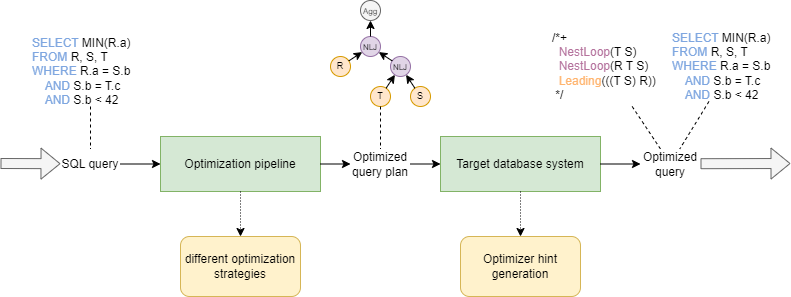
\includegraphics[width=\linewidth]{figures/postbound-workflow.pdf}
	\caption{The basic \emph{PostBOUND} query optimization workflow.}
	\label{fig:postbound-workflow}
\end{figure}

\subsection{Implementation of the Upper Bound Optimization}
\label{sec:postbound-optimization}

The core process in \emph{PostBOUND} is the query optimization loop. 
This loop is designed to work with arbitrary queries and database schemas, as long as some basic criteria are met. 
Specifically, the currently supported queries have to have the following properties:
\begin{compactitem}
    \item each part of the \sql{SELECT} clause is either an attribute or an aggregation of attributes
    \item all joins are either equality predicates over base table attributes, or conjunctions of such predicates
    \item each base table can be filtered using arbitrary predicates that are not optimized further
    \item each query can optionally contain a \sql{GROUP BY}, \sql{ORDER BY}, or \sql{HAVING} clause
\end{compactitem}

Since these properties do not pose any significant restriction on the allowed structure of the query, the optimization algorithm cannot rely on simplifying assumptions. 
Instead, it takes a more general approach by explicitly modeling the \emph{join graph} of the query and using this graph as the central data structure during optimization. 
The join graph $G$ of a query $Q$ is an undirected, colored graph. 
Each base table of $Q$ is represented as a node in $G$ and each join between base tables becomes an edge in the graph. 
Each node is colored as follows: nodes that have not been included in the final join order yet are marked as ``free''. 
As soon as the node has been included in the join order, this color is updated. 
Furthermore, each table is colored by the role it plays in relation to other tables. 
Tables that are exclusively joined via primary key/foreign key joins receive one color and all tables that take part in at least one n:m join receive another color. 
This association can change during an optimization run as former primary key/foreign key tables can become n:m tables if one of their primary key join partners is included in the join tree. 
In addition to colored nodes, the join graph also contains colored edges representing specific joins. 
Each edge is colored by its corresponding join predicate. 
As with table nodes, a second color dimension is used to describe whether the join predicate is a primary key/foreign key join.
In that case, the edge also stores the role each of each partner.

%\begin{figure}[tb]
%	\centering
%	\begin{subfigure}[b]{0.47\textwidth}
%	    \centering
%	    \includegraphics[width=\textwidth]{figures/join-tree-linear.pdf}
%	    \caption{Linear join tree}
%	    \label{fig:join-tree-linear}
%	\end{subfigure}
%	\begin{subfigure}[b]{0.47\textwidth}
%	    \centering
%	    \includegraphics[width=\textwidth]{figures/join-tree-subqueries.pdf}
%	    \caption{Bushy join tree with subquery.}
%	    \label{fig:join-tree-bushy}
%	\end{subfigure}
%	\caption{Different join trees for joining the base tables \sql{A} to \sql{E}. \TODO{polish, caption/subcaption eingebunden - ist das OK?}}
%	\label{fig:join-trees}
%\end{figure}

While the join graph captures the tables that are available for the next join, the \emph{join tree} describes the order in which already selected tables should be joined. 
This is not limited to a strictly linear sequence of joins. 
Instead, a join tree may also contain branches in the form of subqueries 
Thus, the join tree becomes the main result artifact of the query optimization process in \emph{PostBOUND}.

\begin{figure}[tb]
	\centering
	\includegraphics[width=0.3\linewidth]{figures/primary-key-hull.pdf}
	\caption{Primary key hull of table \sql{A}. Tables belonging to the hull are highlighted in blue.}
	\label{fig:primary-key-hull}
\end{figure}

\begin{algorithm}
    \caption{Pseudo-code implementation of the UES algorithm used in \emph{PostBOUND}.}
    \label{alg:postbound}
    \begin{algorithmic}[1]
        \State $join\:graph \gets $ build from $query$
        \State $join\:tree \gets $ empty join tree
        \State
        \State // base estimates, join bounds and subquery generation are subject to flexible policies
        \State // join bounds depend on formula-specific statistics and current upper bounds
        \State
        \If{$join\:graph$ contains only PK/FK joins}
            \State \Return $join\:tree$ according to Algorithm~\ref{alg:postbound-pkfk}
        \EndIf
        \State
        \While{$join\:graph$ contains free n:m joined table}
            \ForAll{free n:m joined tables}
                \State determine minimum bound with free primary key join partners
                \State $upper\_bound(table) = min(primary\:key\:bound,\;base\_estimate(table))$
            \EndFor
            \State
            \If{$join\:tree$ is empty}
                \State $initial\:table \gets$ table with minimum $upper\:bound$
                \State initialize $join\:tree$ with $initial\:table$
                \State include primary key hull of $initial\:table$ in $join\:tree$  \Comment sorted by cardinality estimates
                \State
                \State initialize statistics based on $initial\:table$
                \State mark $initial\:table$ and primary key hull as joined
                \State \textbf{continue}
            \EndIf
            \State
            \ForAll{free n:m joined tables}
                \State determine minimum join bound with $join\:tree$ \Comment using current upper bounds
            \EndFor
            \State
            \State $next\:table \gets$ table with minimum join bound
            \State determine primary key hull of $next\:table$ \Comment sort tables by cardinality estimates
            \If{should generate subquery for $next\:table$ and primary key hull}
                \State insert subquery into $join\:tree$
            \Else
                \State insert $next\_table$ and primary key hull into $join\_tree$
            \EndIf
            \State
            \State updates statistics based on join with $next\:table$
            \State mark $next\:table$ and primary key hull as joined
        \EndWhile
        \State
        \State \Return $join\:tree$
    \end{algorithmic}
\end{algorithm}

Join graph and join tree are the cornerstones of the \emph{PostBOUND} optimization loop. 
A pseudo-code implementation of the \emph{PostBOUND} optimization algorithm is given in Algorithm~\ref{alg:postbound}: During each iteration, the algorithm pulls n:m candidate tables from the join graph and evaluates their current bounds, such that the candidate with minimum bound is inserted into the join tree. 
This selection focuses only on n:m joined tables, because primary key/foreign joins are treated as special filters of the foreign key (and by extension n:m joined) table that can potentially lower the candidate's bound.
Thus, primary key tables are inserted into the join tree together with their foreign key counterpart.
One caveat with this strategy is the existence of primary key tables which are in turn filtered by other primary keys. 
Such tables are also included in the join tree together with their partner. 
In other words, the optimization algorithm includes the entire \emph{hull} of primary key tables when selecting the next table (cf. Figure~\ref{fig:primary-key-hull}). More formally speaking, the \emph{primary key hull} of a table $T$ contains all free tables $R$, such that $R \bowtie S$ is a primary key/foreign key join with $R$ acting as the primary key partner, and $S$ is either equal to $T$ or another table of the primary key hull. Figure~\ref{fig:primary-key-hull} illustrates this concept.

\subsection{Adapting the PostBOUND optimizer}
\label{sec:postbound-optimizer-adapters}

A key difference to the UES optimization loop is the more abstract nature of the \emph{PostBOUND} optimization algorithm: The loop contains a number of adapters where custom behaviour can be injected. These adapters include 

\begin{description}
    \item[Base table estimates] \emph{PostBOUND} does not require a specific strategy to estimate the number of tuples in a (filtered) base table. It only relies on the existence of a numerical estimate and makes no assumption about how this is obtained. Nevertheless, three basic strategies are already provided and new strategies can be injected easily. The provided strategies include: delegating the estimation process to the Postgres-native optimizer, sampling a fraction of the filtered table, or executing the entire filter predicate and counting the result tuples.
    \item[Join bound estimates and statistics] In order to obtain an estimate of the join cardinality, a large number of different strategies have been proposed in recent literature. \emph{PostBOUND} does not restrict the choice of any particular formula, as long as it is capable of estimating the cardinality of any $n$-ary join. Still, the UES formula (see Section~\ref{sec:UES}) and two variations of the Top-k-based formula (see Section~\ref{sec:TighterBounds}) are provided with \emph{PostBOUND}. Since join estimation oftentimes relies on specific \emph{statistical information}, each estimation strategy ships its own tailored implementation. The statistics interface receives update information by the optimization loop.
    \item[Subquery generation] \label{item:postbound-subqueries} Lastly, \emph{PostBOUND} also delegates the decision of when to generate subqueries for primary key/foreign key joins to custom policies. In this case, four strategies are already supplied by default: a greedy strategy that always generates subqueries, a defensive strategy that generates subqueries if they guarantee to reduce the size of the foreign key table (as proposed in \TODO{cite SDR}), a ``smart'' strategy that generates subqueries if a reduction below a certain threshold is guaranteed, and finally a strategy that never generates subqueries at all, thereby leaving all join paths linear
\end{description}

\begin{figure}[tb]
	\centering
	\includegraphics[width=\linewidth]{figures/postbound-interaction.pdf}
	\caption{Interaction between the core \emph{PostBOUND} components for query optimization.}
	\label{fig:postbound-interaction}
\end{figure}

To reiterate, the adapter implementations are not intended to cover all possible scenarios. Instead, they should catch the most common cases and enable user-supplied strategies to replace them as necessary. Figure~\ref{fig:postbound-interaction} summarizes the interaction of the \emph{PostBOUND} optimization algorithm with the various policies. To enable maximum independence from specific workloads or database schemas, all provided components of the \emph{PostBOUND} optimizer query the actual Postgres instance for metadata such as index structures, tuple counts, or attribute value distributions, instead of relying on manual input data.

\begin{algorithm}[tb]
    \caption{Pseudo-code implementation of the heuristic primary key/foreign key join order optimization in \emph{PostBOUND}.}
    \label{alg:postbound-pkfk}
    \begin{algorithmic}[1]
        \State $initial\:table \gets$ foreign key table with minimum base estimate
        \State $join\:tree \gets$ initialized on $initial\:table$
        \State mark $initial\:table$ as joined
        \While{free tables remain}
            \State select free table with minimum base estimate and connection to $join\:tree$
            \State include selected table in $join\:tree$
            \State mark selected table as joined
        \EndWhile
        \State \Return $join\:tree$
    \end{algorithmic}
\end{algorithm}

\begin{algorithm}[tb]
    \caption{Pseudo-code implementation of the cross-product join order optimization in \emph{PostBOUND}.}
    \label{alg:postbound-crossproduct}
    \begin{algorithmic}[1]
        \State $join\:graph \gets$ build from $query$
        \ForAll{$component$ in $join\:graph$}
            \State obtain optimized join order according to Algorithm~\ref{alg:postbound}
        \EndFor
        \State sort component join orders by their final upper bounds
        \State $join\:tree \gets$ build from sorted join orders
        \State \Return $join\:tree$
    \end{algorithmic}
\end{algorithm}

\subsection{...}
\label{sec:postbound-query-extensions}

Other than using custom policies instead of hard-coded formulas, the \emph{PostBOUND} optimization algorithm is also extended to support query structures that surpass the scope of n:m joins, which are the primary focus of UES. Specifically, \emph{PostBOUND} can also handle queries that exclusively consist of primary key/foreign key joins, queries that contain cross products and composite join predicates.

\begin{description}
    \item[Primary key/foreign key queries] To optimize queries that do not contain any n:m join, such as queries on star- or snowflake schemas, a heuristic approach inspired by UES is used. Algorithm~\ref{alg:postbound-pkfk} provides a pseudo-code listing: Since primary key/foreign key joins are guaranteed to never produce more tuples than the cardinality of the foreign key relation, the algorithm starts with the smallest foreign key table and iteratively includes connected tables according to their respective cardinality estimates. This strategy tries to minimize the number of tuples that have to be processed, but only treats the join order as a local optimization problem. An extension that also considers the join cardinalities could be a natural improvement in future work.
    \item[Cross product queries] Queries with cross products are characterized by tables that are neither directly nor indirectly linked with join predicates. Using the join graph this situation can be easily detected through the existence of multiple graph components. Since each of these components represents a complete join graph on its own, an optimized join order can be obtained per partition. Afterwards, a final join order can be constructed by sorting the individual join trees according to their upper bounds. This strategy is summarized in Algorithm~\ref{alg:postbound-crossproduct}.
    \item[Composite join predicates] In contrast to the two previous extensions, composite join predicates do not influence the join order itself. Rather, composite join predicates need to be handled during join cardinality estimation and are therefore subject to the policies. In case of estimators that calculate upper bounds, this case can be handled quite naturally: Since a conjunctive predicate requires each of the individual base predicates to be fulfilled, the final upper bound is constrained by the smallest estimate of the base predicates. Therefore, the upper bound estimator can simply calculate the minimum of base estimates. Other join estimators may rely on different strategies such as the calculation of mean bounds, but for the UES estimator as well as the Top-k estimators the minimum strategy is used.
\end{description}

\subsection{Summary}
\label{sec:postbound-summary}

We introduced \emph{PostBOUND}, our framework to systematically evaluate different approaches to pessimistic query optimization. \emph{PostBOUND} is a PostgreSQL-specific set of components that use a query optimization algorithm adapted from UES. The algorithm enables the adaption of base table estimates, join cardinality estimates and the generation of subqueries. Furthermore, \emph{PostBOUND} is designed to operate without any additional user-supplied data and fetches all required information from the Postgres instance. This enables independence from specific benchmarks and database schemas. Using this framework, we can optimize different workloads and compare their results in a reproducible and transparent way.
